\documentclass{softwaremanual}

\usepackage{titling}

% Figures and controlling packages
\usepackage{float}
\usepackage{wrapfig}

% logo for the title page
\newcommand{\swlogo}{{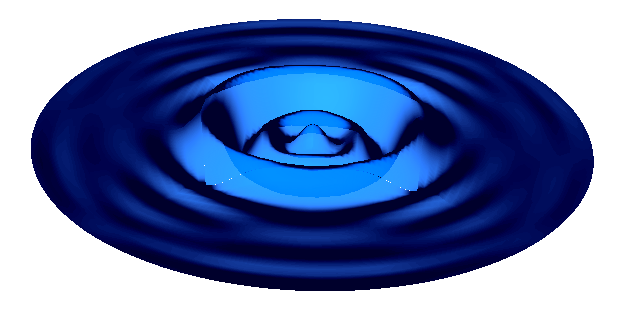
\includegraphics[width=0.25\textwidth]{images/shallowWater.png}}
}


\author{Joseph Schoonover}
\date{}

\begin{document}
\frontmatter
% Doing a custom title-page
\begin{titlingpage}
    
        \vspace*{2cm}

   % Setup up the main and sub-titles with the logo
   {\fontfamily{cmss}\selectfont
   \begin{center}
     \HUGE{\textbf{ Spectral Element Libraries in Fortran (SELF) }}\\

     \huge{\textbf{\textcolor{blue}{Barotropic, Geostrophic Circulation}}}
     \huge{\textit{\textcolor{blue}{Steady State Solver}}}
   \end{center}
    }    
 
        \vspace{1cm}
        
%        \begin{center}
%         \swlogo
%        \end{center}
        
        \vspace{2cm}
        
     \begin{center}
     
        %Do a subtitle here if you like
        {\fontfamily{cmss}\selectfont
        \huge{
           Reference Manual
        }
        
        \vspace{1.5cm}
        
        % Enter the author's name
        \textbf{
        \large{
           \theauthor 
         }}}
        
        \vfill
        
        
     \end{center}
        
    
\end{titlingpage}


{\fontfamily{cmss}\selectfont
\tableofcontents
}
\mainmatter

% Special Style
\pagestyle{myheadings}

\chapter{Equations and Discretization}
The dynamics of the large scale oceanic circulation on earth are largely contained within the hydrostatic primitive equations. In these equations, the vertical momentum balance is approximated by hyrdostatic balance - an approximation that is justified by the use of the ``thin shell'' approximation, where the fluid depth is far smaller than the lateral length scales of motion. For a constant density fluid, the hydrostatic primitive equations can be reduced to the shallow water equations, so long as the effects of thin boundary layers are parameterized. For sufficiently slow moving flows, the effects of gravity waves can be approximated as instantaneous adjustments of the fluid surface that act to keep the fluid transport divergence free; this is known as the rigid lid assumption. Steady state, linear flows subject to all of the previous assumptions are now governed by two equations :
\begin{subequations}
\begin{align}
  f \hat{z} \times \vec{u} &= \nabla P + \frac{ \vec{\tau} }{H} - \frac{C_d \vec{u}}{H} \\
  \nabla \cdot \left( H \vec{u} \right) &= 0.
\end{align}\label{eq:eqofmotion}
\end{subequations}
In Eqs. \eqref{eq:eqofmotion}, $f$ is the coriolis parameter, $\vec{u} = u \hat{x} + v\hat{y}$ is the lateral velocity field, $P$ is the barotropic fluid pressure, $\vec{\tau}$ is the stress imposed on the fluid at the surface, $C_d\vec{u}$ is a parameterization of the stress felt at the sea-floor, $C_d$ is a drag coefficient, and $H$ is the fluid depth.

Eq. (\ref{eq:eqofmotion}b) is satisfied exactly if the transport is written in terms of a stream function
\begin{equation}
H \vec{u} = \hat{z} \times \nabla \Psi. \label{eq:stream}
\end{equation}
Further, the equation set \eqref{eq:eqofmotion} can be reduced to a single equation for the stream function by taking the curl of (\ref{eq:eqofmotion}a) and substituting in \eqref{eq:stream}. Doing so gives
\begin{equation}
 \nabla \cdot \left( \frac{C_d \nabla \Psi}{H^2} \right) + \nabla \Psi \times \nabla Q = \nabla \times \left( \frac{\vec{\tau}}{H} \right) ,\label{eq:eqsolved}
\end{equation} 
where 
\begin{equation}
Q = \frac{f}{H}
\end{equation}
is the background potential vorticity.


\section{Nodal Continuous Galerkin Discretization}


\section{Iterative Solution Technique}
The discretized drag operator is symmetric, while the potential vorticity advection operator is asymmetric. Overall, the system is asymmetric. Previous implementation of the SELF-CGSEM solver make use of the preconditioned conjugate gradient method, an iterative solver that is not directly applicable to asymmetric systems. Here, GMRES is used to find solutions to \eqref{eq:eqsolved}.


\chapter{Learning to Walk}
The ``Stommel'' solver, which solves equation \eqref{eq:eqsolved} subject to Dirichlet boundary conditions, is included in the set of ``highend'' solvers of the SELF. Right now, the easiest way to obtain the code is to download the most recent snapshot of the SELF from \href{https://github.com/schoonovernumerics/SELF}{the github repository}. The easiest way to get started is to learn how to download, compile, run, and configure a pre-built and tested example included with the software (e.g. $\sim$/SELF/examples/Stommel/WindDrivenGyre/). The easiest way to view the output from the example (and your future modified implementations) is to use a GUI that can read \textit{tecplot} files, such as \href{https://wci.llnl.gov/simulation/computer-codes/visit/}{VisIt} (Note that the native output of the SELF is in tecplot format). This section of the documentation will walk you through how to use the code in the easiest way possible ( or so I would think ), using the workflow that I've grown into over the last few years as the SELF has developed.


\section{Downloading}
The SELF is currently available on a github. There are two ways to obtain the code. If you are interested in obtaining the most recent snapshot of the code, a tar file can be downloaded directly from the git website.  \href{https://github.com/schoonovernumerics/SELF}{Clicking here will bring you to the SELF.} Once you follow the link ( if the embedded link doesn't work, copy and paste
\begin{verbatim}
 https://github.com/schoonovernumerics/SELF 
\end{verbatim}
into your browser's url bar ) click on ``Download ZIP'', which is located towards the right side of the page. Unpack the tar file into your favorite directory. This will make a directory ``SELF'' in your favorite directory, underneath which all of the source code and examples included with the SELF. 

Alternatively, if you have git installed on your computer, you can clone the SELF repository by issuing the command
\begin{center}
\begin{verbatim}
git clone https://github.com/schoonovernumerics/SELF
\end{verbatim}
\end{center}
Again, this will make the directory ``SELF'' in the current directory where you issued the clone command. 

\section{Compile the example}
At this point, you should have downloaded the SELF. We will first navigate to the examples directory and find the example for the wind-driven gyre demo. This example can be found under
\begin{center}
\begin{verbatim}
SELF/examples/Stommel/WindDrivenGyre/
\end{verbatim}
\end{center}
Go ahead and change directories to the wind-driven gyre example.

As with all of the supplied examples, there are three subdirectories
\begin{center}
\begin{verbatim}
build/     localmods/    run/
\end{verbatim}
\end{center}
This subdirectory structure is used in order to keep your model output, source code modifications, and model build details separate. For now we won't worry about the \texttt{localmods/} subdirectory; this subdirectory will be discussed later in Sec. \ref{sec:config} where we will illustrate how to modify the source code if needed for your application.

Right now, the most important thing is to get you familiar with compiling and running the code. Change directories into the build subdirectory. Underneath the build directory, there is a makefile and a simple build script. For now, you don't need to worry about changing anything to either one of these files. In Sec. \ref{sec:config}, there are directions for changing your fortran compiler, compiler optimizations, warning flags, debugging flags, etc. To compile the code, simply type the command
\begin{verbatim}
./rebuild.sh
\end{verbatim}
and press enter. This will compile all of the necessary modules and the driver program needed to create the \texttt{stommel} executable (all of these dependencies are expressed in the makefile). Additionally, the \texttt{rebuild} script cleans up the build directory by removing the \texttt{.o} and \texttt{.mod} files and moves the executable to the run directory. If you have problems running the build script, it may be that the permissions are not set appropriately. To set the proper permissions, do
\begin{verbatim}
chmod 755 rebuild.sh
\end{verbatim}
and then try to run the script again. If this still doesn't work, send me an e-mail, and issue the commands
\begin{verbatim}
make stommel
make clean
mv stommel ../run/
\end{verbatim}

\section{Running the Code and Viewing the Output}
Ok, so now you have successfully compiled the code. Change directories to the \texttt{run} directory. In the run directory, you will find the executable (\texttt{stommel}) and a text file, \texttt{runtime.params}.

\subsection{Running the Code}
The \texttt{stommel} executable requires that you have a namelist file in the directory named \texttt{runtime.params}. There should be one included already with your fresh download. This namelist file specifies parameters that are used for the iterative solver, spatial discretization, plotting, and setting physical parameters for the barotropic vorticity model. For the moment, feel free to take a look at the file to familiarize yourself with the parameters, but don't worry about setting anything; the provided parameters file yields a successful run for Stommel's wind-driven gyre. In Sec. \ref{sec:config}, we will discuss each parameter.

To run the code, issue the command
\begin{verbatim}
./stommel
\end{verbatim}
Doing so, will solve a CGSE discretized version of \eqref{eq:eqofmotion} subject to homogeneous Dirichlet boundary conditions. Once it finishes running, there will be three files that are generated:
\begin{enumerate}
\item \texttt{mesh.tec} : A tecplot file that contains the computational mesh and metric terms that were used in the computation of the solution.
\item \texttt{CGsemSol.tec} : A tecplot file that contains the solution, mapped to uniform points within each spectral element. The solution variables include the transport stream function and transport field \texttt{(U, V)}. Additionally, the fluid depth, coriolis parameter, and any source terms are reported in this file.
\item \texttt{residual.curve} : The residual at each step of the GMRES iterative solver. If you are ``tuning'' the iterative solver for a new configuration, monitoring the residual may be provide some guidance.
\end{enumerate}

Now that the code has finished running and you have some output, you can view the tecplot and curve files in your favorite visualization software. Here, we will describe how to view the output using \href{https://wci.llnl.gov/simulation/computer-codes/visit/}{VisIt}.

\subsection{Viewing the output in VisIt}
\section{Configuration}\label{sec:config}
\clearpage

\appendix

\chapter{Spectral Element Primer}

\section{Vector Spaces}


\section{Spectral Approximations and Error Analysis}

\chapter{Differential Geometry}\label{chap:GeometryTheory}

\pagebreak

\bibliography{hpe-refs}
\bibliographystyle{plainnat}
\end{document}